\subsection{x86}

\subsubsection{\NonOptimizing MSVC}

\RU{Имеем в итоге}\EN{We get} (MSVC 2010):

\lstinputlisting[caption=MSVC 2010]{patterns/14_bitfields/2_set_reset/set_reset_msvc.asm}

\index{x86!\Instructions!OR}
\RU{Инструкция \OR здесь устанавливает в переменной ещё один бит, игнорируя остальные.}
\EN{The \OR instruction sets one bit to value while ignoring the rest.}

\index{x86!\Instructions!AND}
\RU{А \AND сбрасывает некий бит. Можно также сказать, что \AND здесь копирует все биты, кроме одного. 
Действительно, во втором операнде \AND выставлены в единицу те биты, которые нужно сохранить, 
кроме одного, копировать который мы не хотим (и который 0 в битовой маске).
Так проще понять и запомнить.}
\EN{\AND resets one bit. It can be said that \AND just copies all bits except one.
Indeed, in the second \AND operand only the bits that need to be saved are set,
just the one do not want to copy is not (which is 0 in the bitmask).
It is the easier way to memorize the logic.}

\ifdefined\IncludeOlly
\clearpage
\myparagraph{\olly}

\RU{Попробуем этот пример в}\EN{Let's try this example in} \olly.
\RU{Сначала, посмотрим на двоичное представление используемых нами констант}
\EN{First, let's see the binary form of the constants we are going to use}:

\TT{0x200} (0000000000000000000{\color{red}1}000000000) 
(\RU{т.е. 10-й бит (считая с первого)}\EN{i.e., the 10th bit (counting from 1st)}).

\RU{Инвертированное}\EN{Inverted} \TT{0x200} \RU{это}\EN{is} \TT{0xFFFFFDFF} 
(1111111111111111111{\color{red}0}111111111).

\TT{0x4000} (00000000000000{\color{red}1}00000000000000) (\RU{т.е. 15-й бит}\EN{i.e., the 15th bit}).

\RU{Входное значение это}\EN{The input value is}: \TT{0x12340678} (10010001101000000011001111000).
\RU{Видим, как оно загрузилось}\EN{We see how it's loaded}:

\begin{figure}[H]
\centering
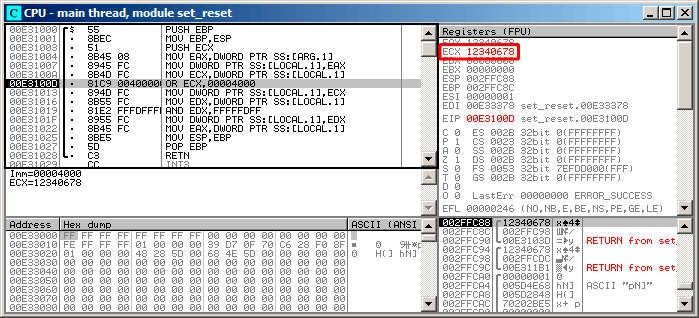
\includegraphics[scale=\FigScale]{patterns/14_bitfields/2_set_reset/olly1.png}
\caption{\olly: \EN{value is loaded into}\RU{значение загружено в} \ECX}
\label{fig:set_reset_olly1}
\end{figure}

\clearpage
\OR \RU{исполнилась}\EN{got executed}:

\begin{figure}[H]
\centering
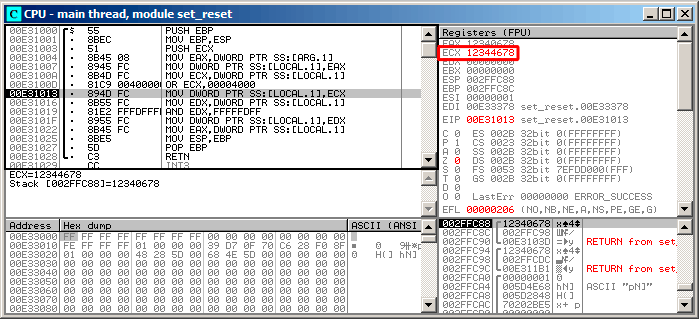
\includegraphics[scale=\FigScale]{patterns/14_bitfields/2_set_reset/olly2.png}
\caption{\olly: \OR \RU{сработал}\EN{executed}}
\label{fig:set_reset_olly2}
\end{figure}

\RU{15-й бит выставлен}\EN{15th bit is set}: \TT{0x1234{\color{red}4}678} 
(10010001101000{\color{red}1}00011001111000).

\clearpage
\RU{Значение перезагружается снова (потому что использовался режим компилятора без оптимизации)}\EN{The value is 
reloaded again (because the compiler is not in optimizing mode)}: 

\begin{figure}[H]
\centering
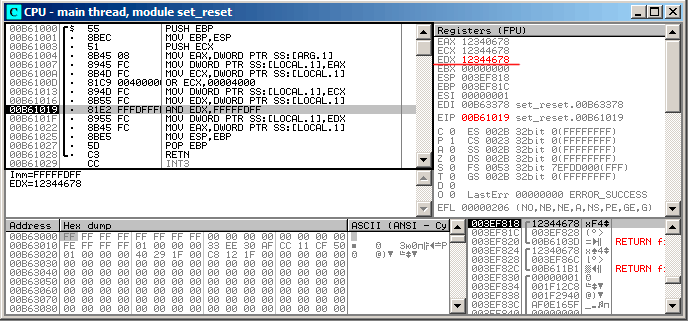
\includegraphics[scale=\FigScale]{patterns/14_bitfields/2_set_reset/olly3.png}
\caption{\olly: \EN{value was reloaded into}\RU{значение перезагрузилось в} \EDX}
\label{fig:set_reset_olly3}
\end{figure}

\clearpage
\AND \RU{исполнилась}\EN{got executed}:

\begin{figure}[H]
\centering
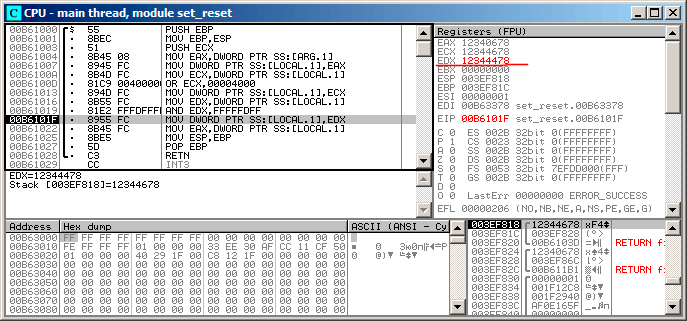
\includegraphics[scale=\FigScale]{patterns/14_bitfields/2_set_reset/olly4.png}
\caption{\olly: \AND \RU{сработал}\EN{executed}}
\label{fig:set_reset_olly4}
\end{figure}

\RU{10-й бит очищен (или, иным языком, оставлены все биты кроме 10-го) и итоговое значение это}
\EN{The 10th bit was cleared (or, in other words, all bits were left except the 10th) and the final value now is} \\
\TT{0x12344{\color{red}4}78} (1001000110100010001{\color{red}0}001111000).

\fi

\subsubsection{\Optimizing MSVC}

\RU{Если скомпилировать в MSVC с оптимизацией (\Ox), то код еще короче:}
\EN{If we compile it in MSVC with optimization turned on (\Ox), the code is even shorter:}

\lstinputlisting[caption=\Optimizing MSVC]{patterns/14_bitfields/2_set_reset/set_reset_msvc_Ox.asm}

\ifdefined\IncludeGCC
\subsubsection{\NonOptimizing GCC}

\RU{Попробуем GCC 4.4.1 без оптимизации:}\EN{Let's try GCC 4.4.1 without optimization:}

\lstinputlisting[caption=\NonOptimizing GCC]{patterns/14_bitfields/2_set_reset/set_reset_gcc.asm}

\RU{Также избыточный код, хотя короче, чем у MSVC без оптимизации.}
\EN{There is a redundant code present,
however, it is shorter than the MSVC version without optimization.}

\RU{Попробуем теперь GCC с оптимизацией}\EN{Now let's try GCC with optimization turned on} \Othree:

\subsubsection{\Optimizing GCC}

\lstinputlisting[caption=\Optimizing GCC]{patterns/14_bitfields/2_set_reset/set_reset_gcc_O3.asm}

\RU{Уже короче. Важно отметить, что через регистр \AH компилятор работает с частью регистра \EAX. 
Это его часть от 8-го до 15-го бита включительно.}
\EN{That's shorter.
It is worth noting the compiler works with the \EAX register part via the \AH 
register---that is the \EAX register part from the 8th to the 15th bits included.}

\RegTableOne{RAX}{EAX}{AX}{AH}{AL}

\index{Intel!8086}
\index{Intel!80386}
N.B. \RU{В 16-битном процессоре 8086 аккумулятор имел название \AX 
и состоял из двух 8-битных половин~--- \AL (младшая часть) и \AH (старшая). 
В 80386 регистры были расширены до 32-бит, 
аккумулятор стал называться \EAX, но в целях совместимости, к его \IT{более старым} частям всё ещё можно 
обращаться как к \AX/\AH/\AL.}
\EN{The 16-bit CPU 8086 accumulator was named \AX and consisted of two 8-bit 
halves---\AL (lower byte) and \AH (higher byte).
In 80386 almost all registers were extended to 32-bit, the accumulator was named \EAX, 
but for the sake of compatibility,
its \IT{older parts} may be still accessed as \AX/\AH/\AL.}

\RU{Из-за того, что все x86 процессоры~--- наследники 16-битного 8086, эти \IT{старые} 16-битные опкоды короче 
нежели более новые 32-битные. 
Поэтому инструкция \INS{or ah, 40h} занимает только 3 байта. 
Было бы логичнее сгенерировать здесь \INS{or eax, 04000h}, но это уже 5 байт, или даже 6 
(если регистр в первом операнде не \EAX).}
\EN{Since all x86 CPUs are successors of the 16-bit 8086 CPU, these \IT{older} 16-bit opcodes are shorter 
than the newer 32-bit ones.
That's why the \INS{or ah, 40h} instruction occupies only 3 bytes.
It would be more logical way to emit here \INS{or eax, 04000h}
but that is 5 bytes, or even 6
(in case the register in the first operand is not \EAX).}

\subsubsection{\Optimizing GCC \AndENRU regparm}

\RU{Если мы скомпилируем этот же пример не только с включенной оптимизацией \Othree, 
но ещё и с опцией \TT{regparm=3}, о которой я писал немного выше, то получится ещё короче:}
\EN{It would be even shorter if to turn on the \Othree optimization flag and also set \TT{regparm=3}.}

\lstinputlisting[caption=\Optimizing GCC]{patterns/14_bitfields/2_set_reset/set_reset_gcc_O3_regparm3.asm}

\index{Inline code}
\RU{Действительно~--- первый аргумент уже загружен в \EAX, и прямо здесь можно начинать с ним работать. 
Интересно, что и пролог функции (\INS{push ebp / mov ebp,esp}) и эпилог (\INS{pop ebp}) 
функции можно смело выкинуть за ненадобностью, 
но возможно GCC ещё не так хорош для подобных оптимизаций по размеру кода. 
Впрочем, в реальной жизни подобные короткие функции лучше всего автоматически делать в виде 
\IT{inline-функций} (\myref{inline_code}).}
\EN{Indeed, the first argument is already loaded in \EAX, so it is possible to work with it in-place.
It is worth noting that both the function prologue (\INS{push ebp / mov ebp,esp}) and epilogue (\INS{pop ebp})
can easily be omitted
here, but GCC probably is not good enough to do such code size optimizations.
However, such short functions are better to be \IT{inlined functions} (\myref{inline_code}).}
\fi
